\documentclass[12pt]{article}

\usepackage{graphicx}
\graphicspath{{../Fichier_Image}}

\title{Hypothèse 5.Taille Bureaux}
\author{Thibault Clodion}

\begin{document}

\maketitle % Permet d'afficher le titre, l'author etc

\underline{Hypothèse :} La taille des bureaux influe sur le temps de sortie (comme vu exp 1. +
4.-7.)
\newline\newline
\underline{Observations déjà faite :}
\newline
$\hspace*{0.2cm}$- Il ne faut pas contraindre la taille des bureaux a des bureaux trop petits (exp 4.) cela fait qu'il y a peu de chemins
et que tout le monde se retrouve à se pousser dans les couloirs
\newline
$\hspace*{0.2cm}$- Il ne faut pas avoir de trop gros bureaux (1.) cela génère de trop gros flux à leur sortie.(on se retrouve presque dans les premières simulations 250 desk uniforme)
\newline
$\hspace*{0.2cm}$- En ayant des bureaux de tailles raisonnables (7.) on obtient un meilleur temps car à la fois on divise les flux importants en sortie de bureau
et on peut en même temps orienté les flux plus facilement.
\newline\newline
\underline{Expérience :}
\newline
5, 10, 15, 20, 25, 30, 35, 40, 45, 50, 55 personnes par bureaux (au max car je peux pas faire tous bureaux taille unique mais on pousse au maximum la taille) 
pour essayer d'observer une gaussienne et conclure sur le nombre de personnes par bureaux qu'il faut au max.
\newline\newline

\section{Expériences}

5. 5 personnes max
\newline\newline
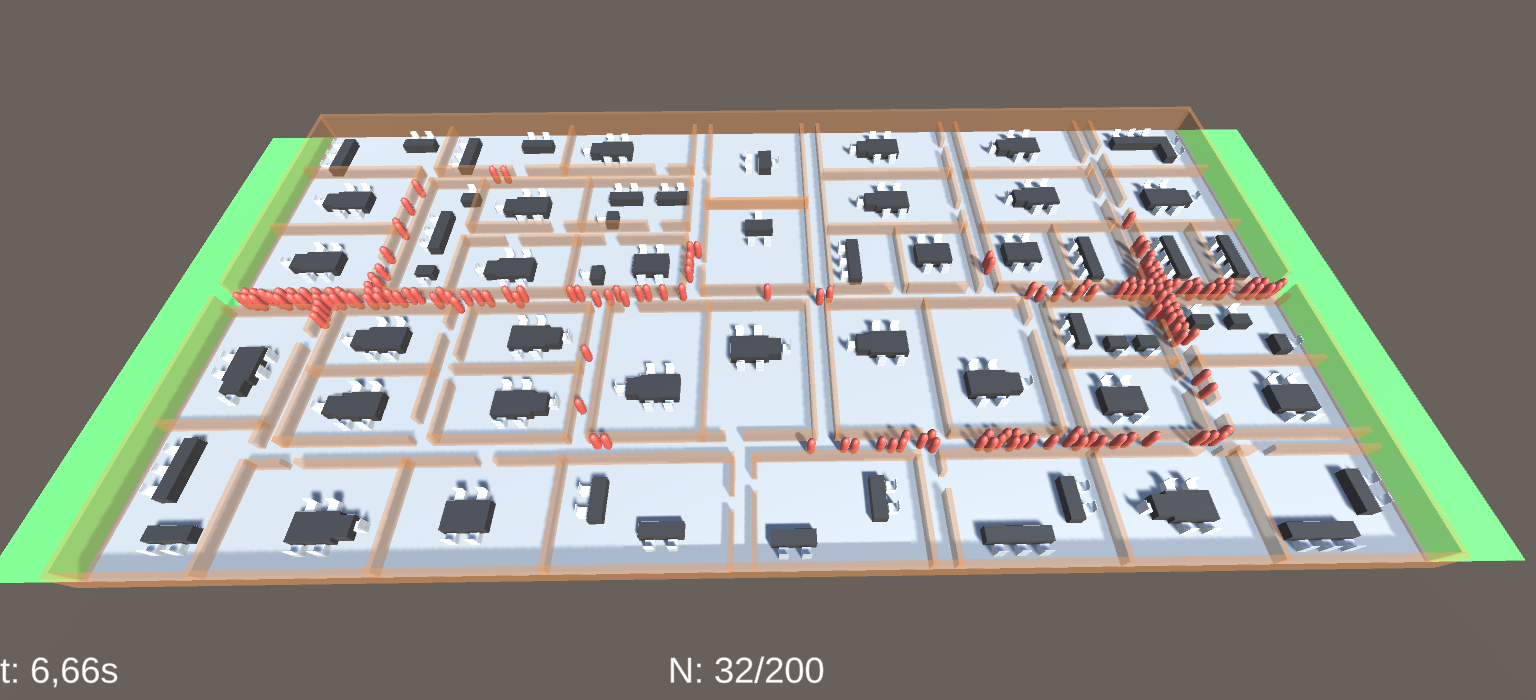
\includegraphics[scale=0.3]{5. 5 personnes max.png}
\newline\newline
Temps moyen de dernière sortie : 24.77
\newline
$\hspace*{0.2cm}$- Grand bloquage au niveau du croisement à droite car on ne peut pas éviter le carrefour étant donné la taille des bureaux imposés.
\newline
$\hspace*{0.2cm}$- Peu de bureau = Peu de contrôle des flux
\newline\newline

5. 10 personnes max
\newline\newline
Temps moyen de dernière sortie : 23.78
\newline
$\hspace*{0.2cm}$- On est relativement sur les mêmes problématiques malgrés quelques améliorations.
\newline\newline

5. 15 personnes max
\newline\newline
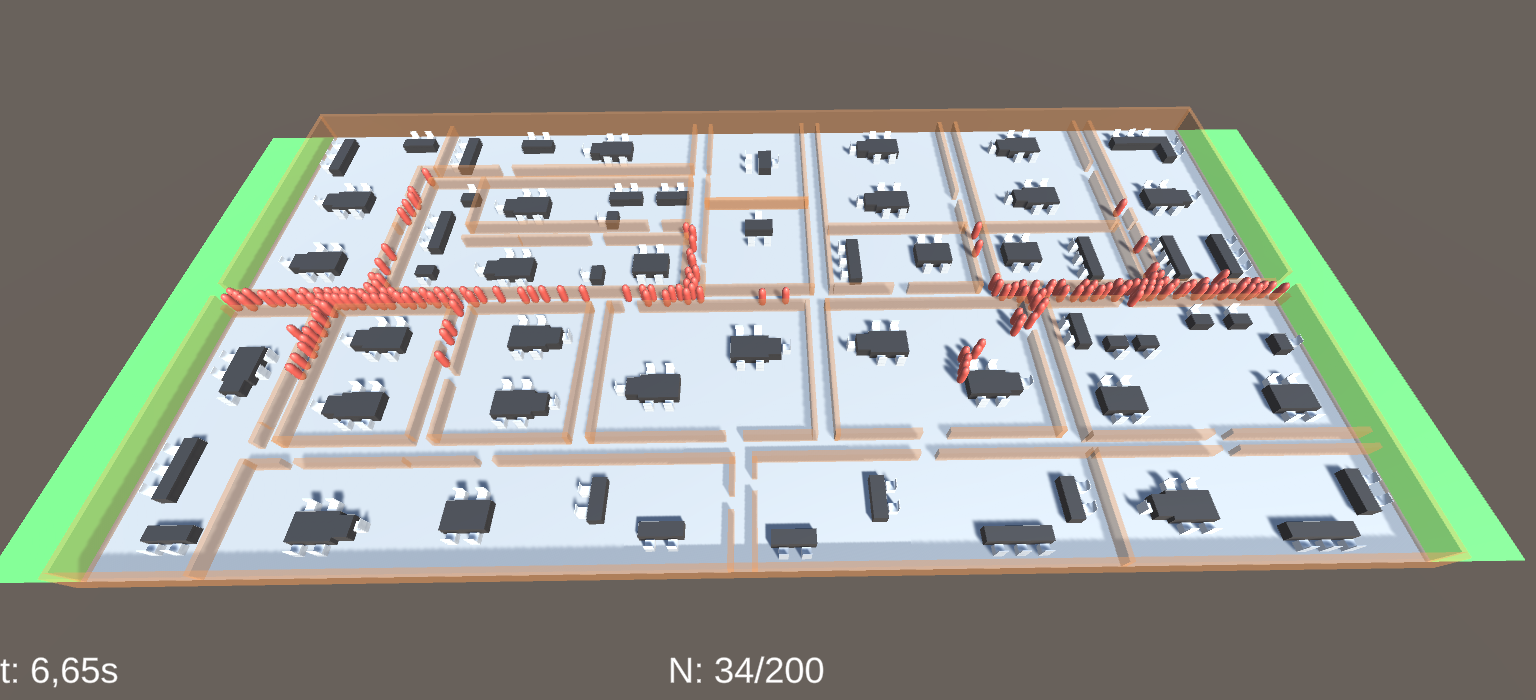
\includegraphics[scale=0.3]{5. 15 personnes max.png}
\newline\newline
Temps moyen de dernière sortie : 22.53
\newline
$\hspace*{0.2cm}$- On peut enfin éviter le carrefour à droite, car la taille des bureaux permets une plus grande modulation des flux.
\newline
$\hspace*{0.2cm}$-On a toujours de grand flux qui se rencontrent mais on a facilement pu contrôler les flux.
\newline\newline

5. 20 personnes max
\newline\newline
Temps moyen de dernière sortie : 22.01
\newline
$\hspace*{0.2cm}$- Encore une facilitation du contrôle des flux.
\newline\newline

5. 25 personnes max
\newline\newline
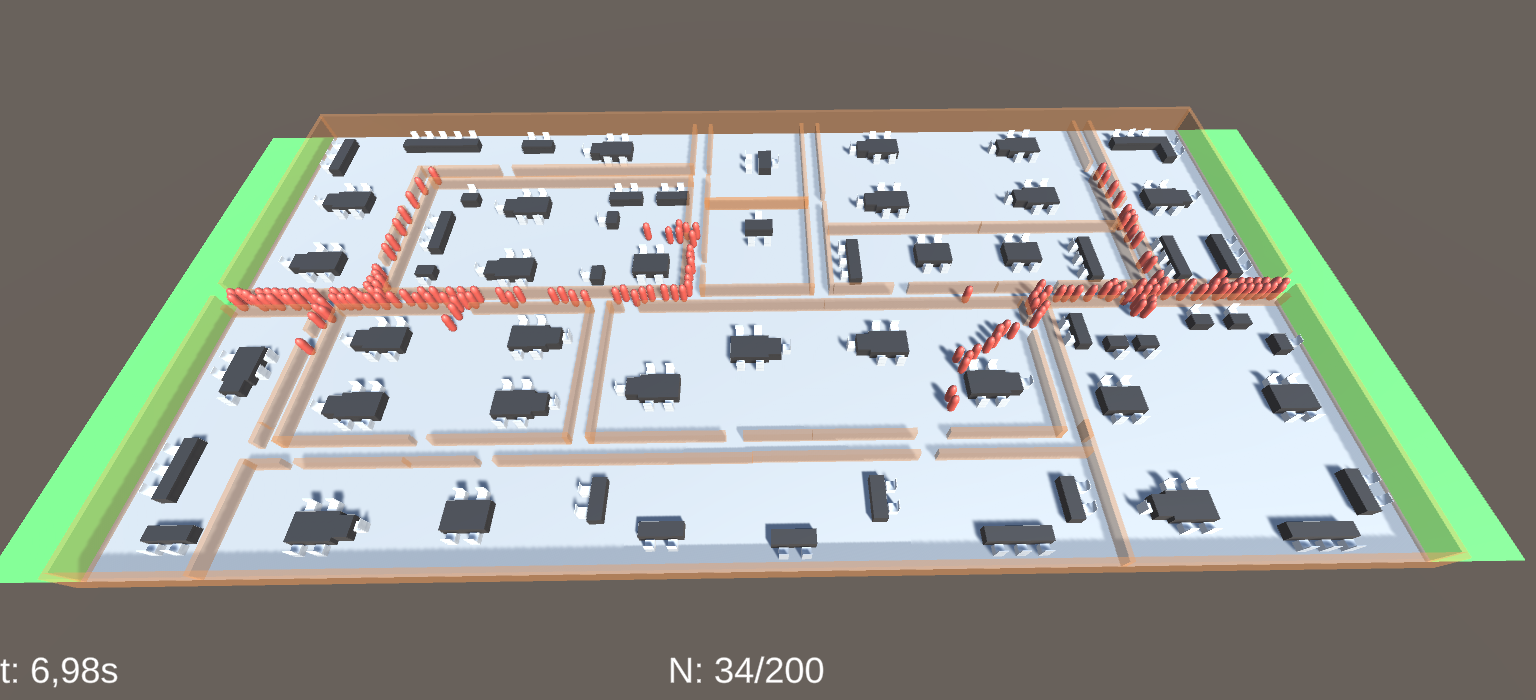
\includegraphics[scale=0.3]{5. 25 personnes max.png}
\newline\newline
Temps moyen de dernière sortie : 23.42
\newline
$\hspace*{0.2cm}$- Le problème se trouve dans le fait que malgré un contrôle des flux, tout le monde commence à emprunter le même chemin.
\newline\newline

5. 30 personnes max
\newline\newline
Temps moyen de dernière sortie : 23.10
\newline
$\hspace*{0.2cm}$- Le temps baisse un peu car la gestion des flux en haut à droite est facilité par des bureaux plus grand.
\newline\newline

5. 40 personnes max
\newline\newline
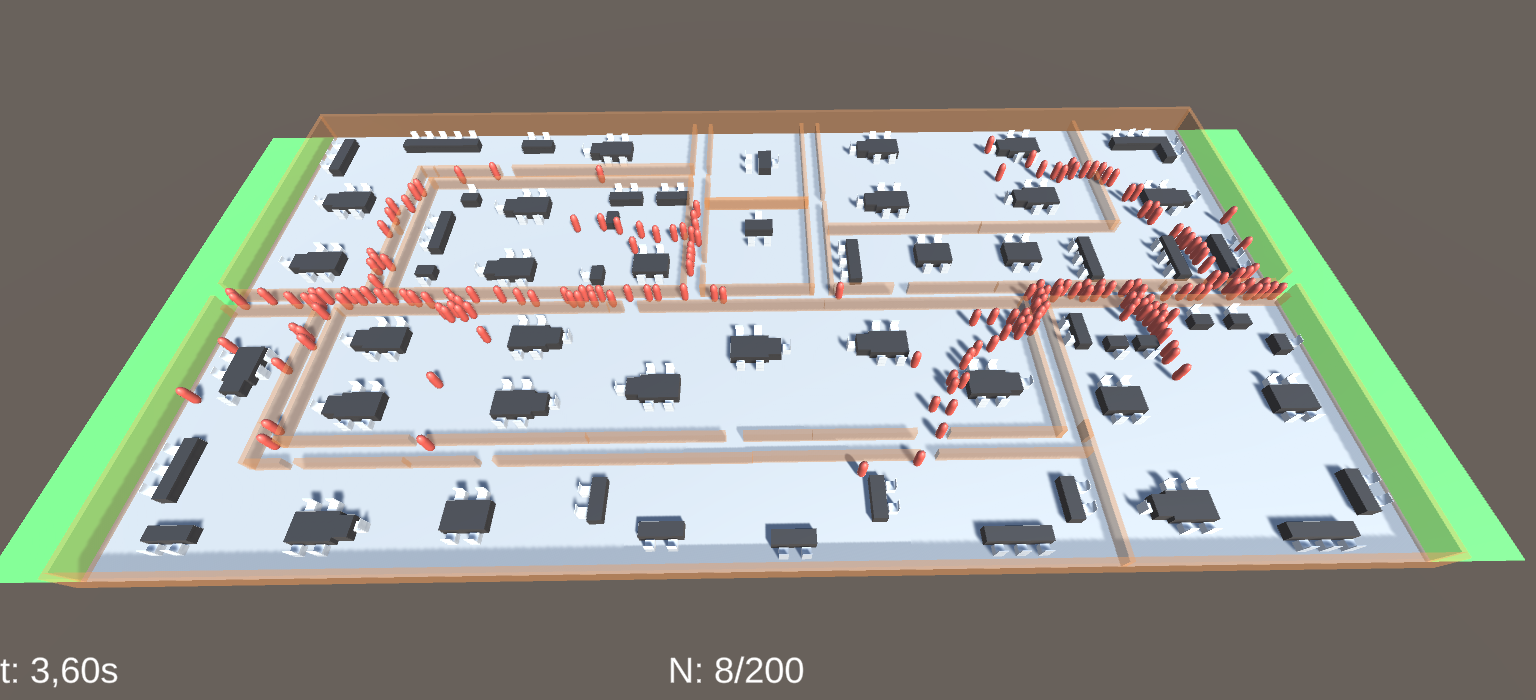
\includegraphics[scale=0.3]{5. 40 personnes max.png}
\newline\newline
Temps moyen de dernière sortie : 22.69
\newline
$\hspace*{0.2cm}$- L'ouverture du bureau au milieu (comme le disait l'hypothèse 3.(a)) est intéressante, elle permet de séparer les flux en offrant plus de chemins.
\newline\newline


5. 50 personnes max (Meilleur temps moyen de sortie)
\newline\newline
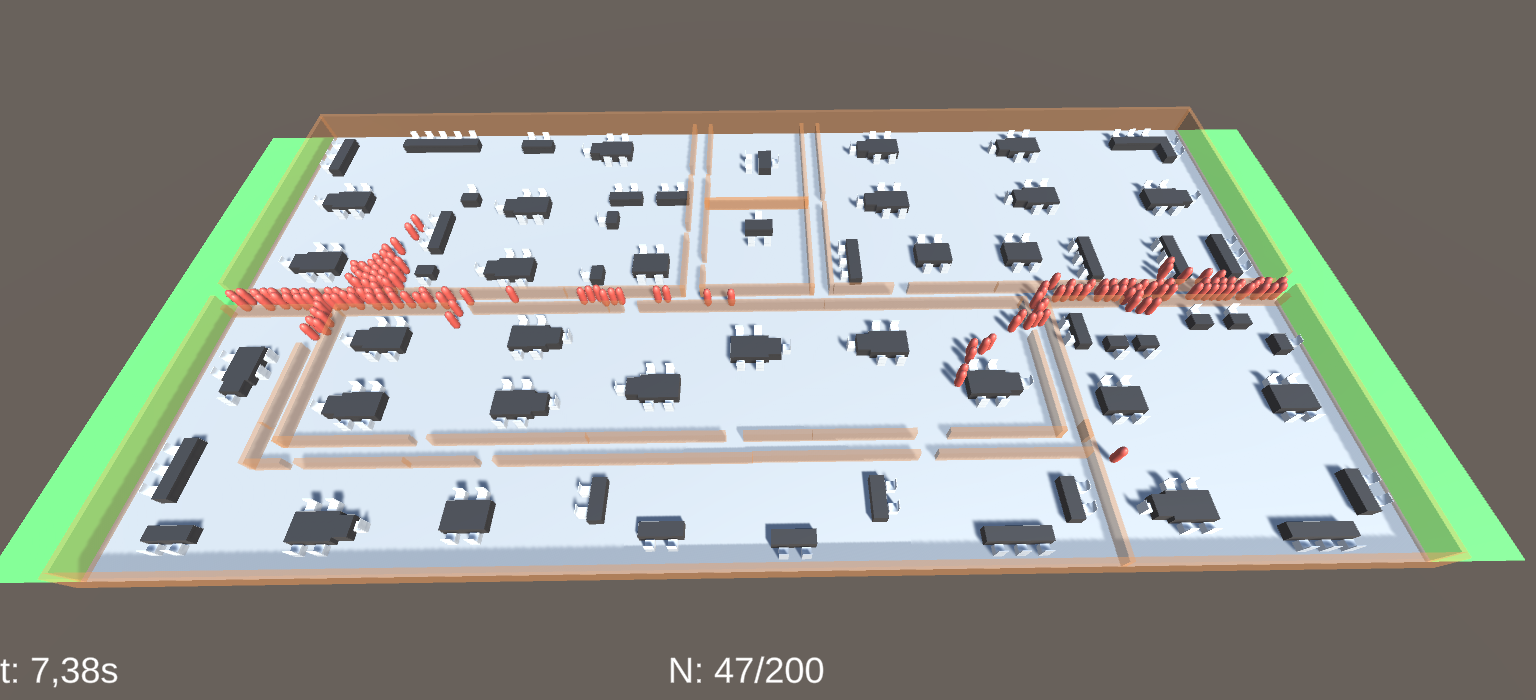
\includegraphics[scale=0.3]{5. 50 personnes max.png}
\newline\newline
Temps moyen de dernière sortie :21.59
\newline
$\hspace*{0.2cm}$- On a des grand flux (dans chaque bureau car ils sont très grands) mais ils se divisent plutôt bien et se confrontent mais relativement peu. (comparé autres simulations)
\newline
$\hspace*{0.2cm}$- Donc finalement le fait de pouvoir contrôler les flux est si intéressant que cela peut être profitable d'avoir des grands bureaux.
\newline\newline

5. 55 personnes max
\newline\newline
Temps moyen de dernière sortie : 22.25
\newline
$\hspace*{0.2cm}$- Il n'y a pas d'amélioration car le fait d'avoir enlever la cloison en bas à droite, fait qu'il y a plus de flux dans le bureau de droite
et moins de flux dans ce qui arrive de la gauche (pour aller à droite)
\newline
$\hspace*{0.2cm}$- Donc au final le temps est plus long.
\newline\newline

5. 100 personnes max
\newline\newline
Temps moyen de dernière sortie :25.97
\newline
$\hspace*{0.2cm}$- Ici on a enlever tous les murs (il reste deux grand bureaux un en bas un en haut)
\newline
$\hspace*{0.2cm}$- On espère evidemment de gros embouteillages à la sortie de chaque bureau étant donné qu'ils sont grand, ce qui ralentit la sortie.

\section{Conclusion}
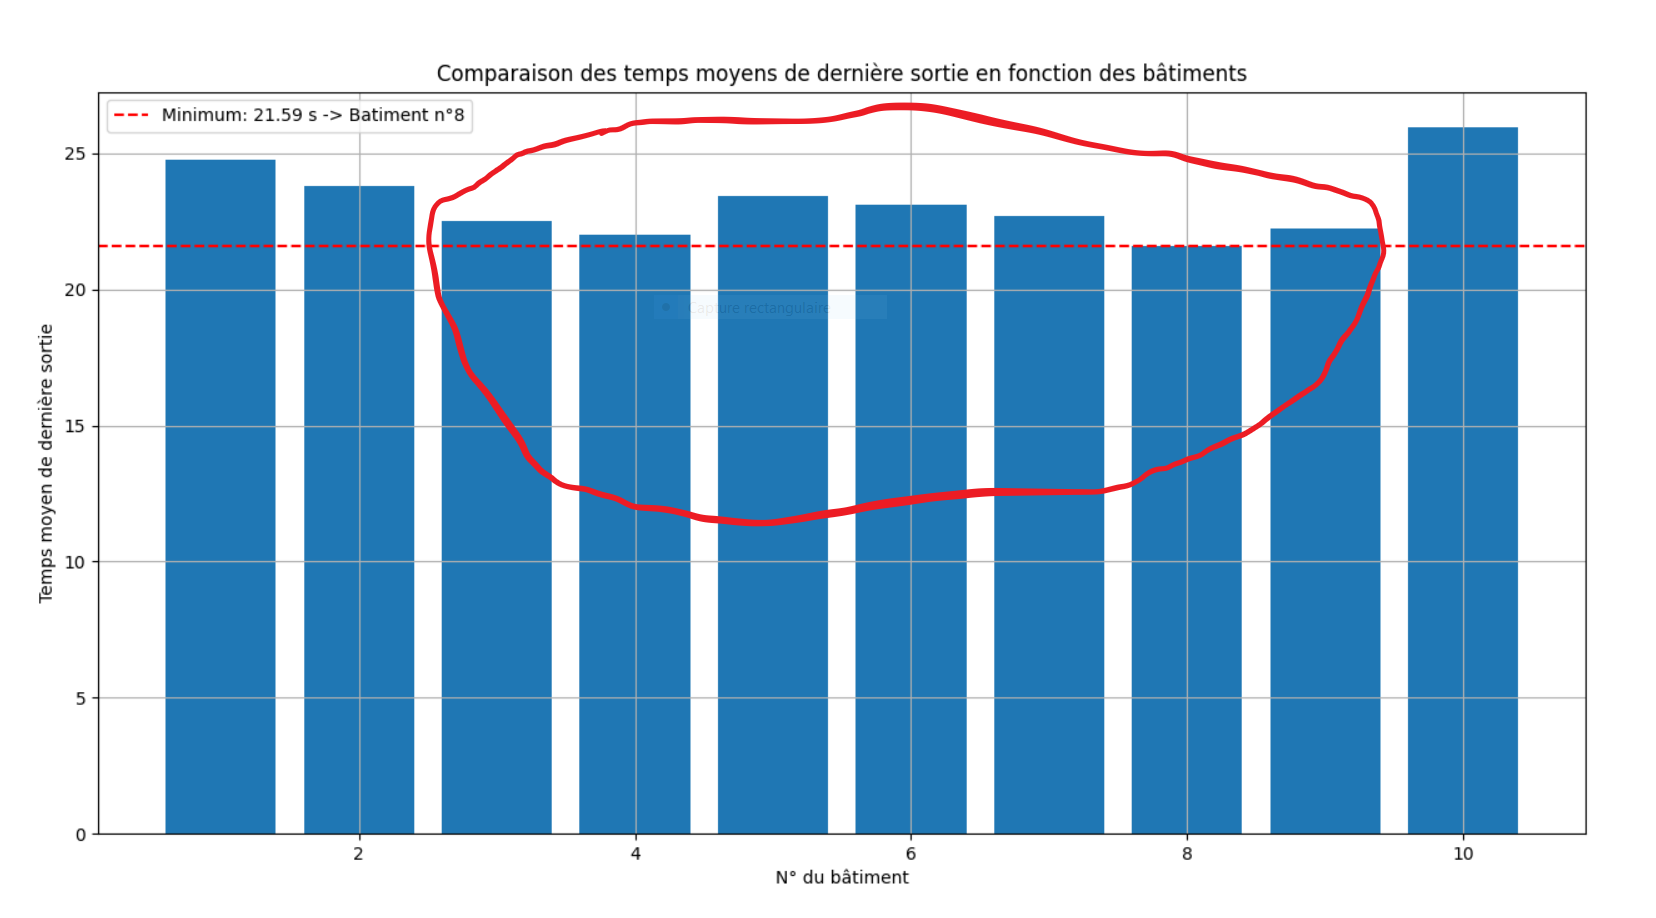
\includegraphics[scale=0.3]{5. Resultat.png}
\newline\newline

On n'observe pas une gaussienne inversé comme attendue. (on ne peut donc pas conclure aussi vite que l'hypothèse)
\newline\newline
Cependant ce qu'on peut tout de même conclure, c'est que pour avoir des temps de sorties meilleurs, il faut avoir des bureaux de taille entre 15 et 55 personnes
(plus ou moins fait augmenter le temps).
\newline
On peut constater que les pires temps se situent pour la taille 5 et la taille 100.
\newline\newline
On conclut donc qu'il faut des bureaux de tailles raisonnables (pas trop grand ni trop petit).



\end{document}